% !TEX root = mythesis.tex

%==============================================================================
\chapter{The Pierre Auger Observatory}
\label{sec:setup}
%==============================================================================
\begin{figure}[h!]
\centering
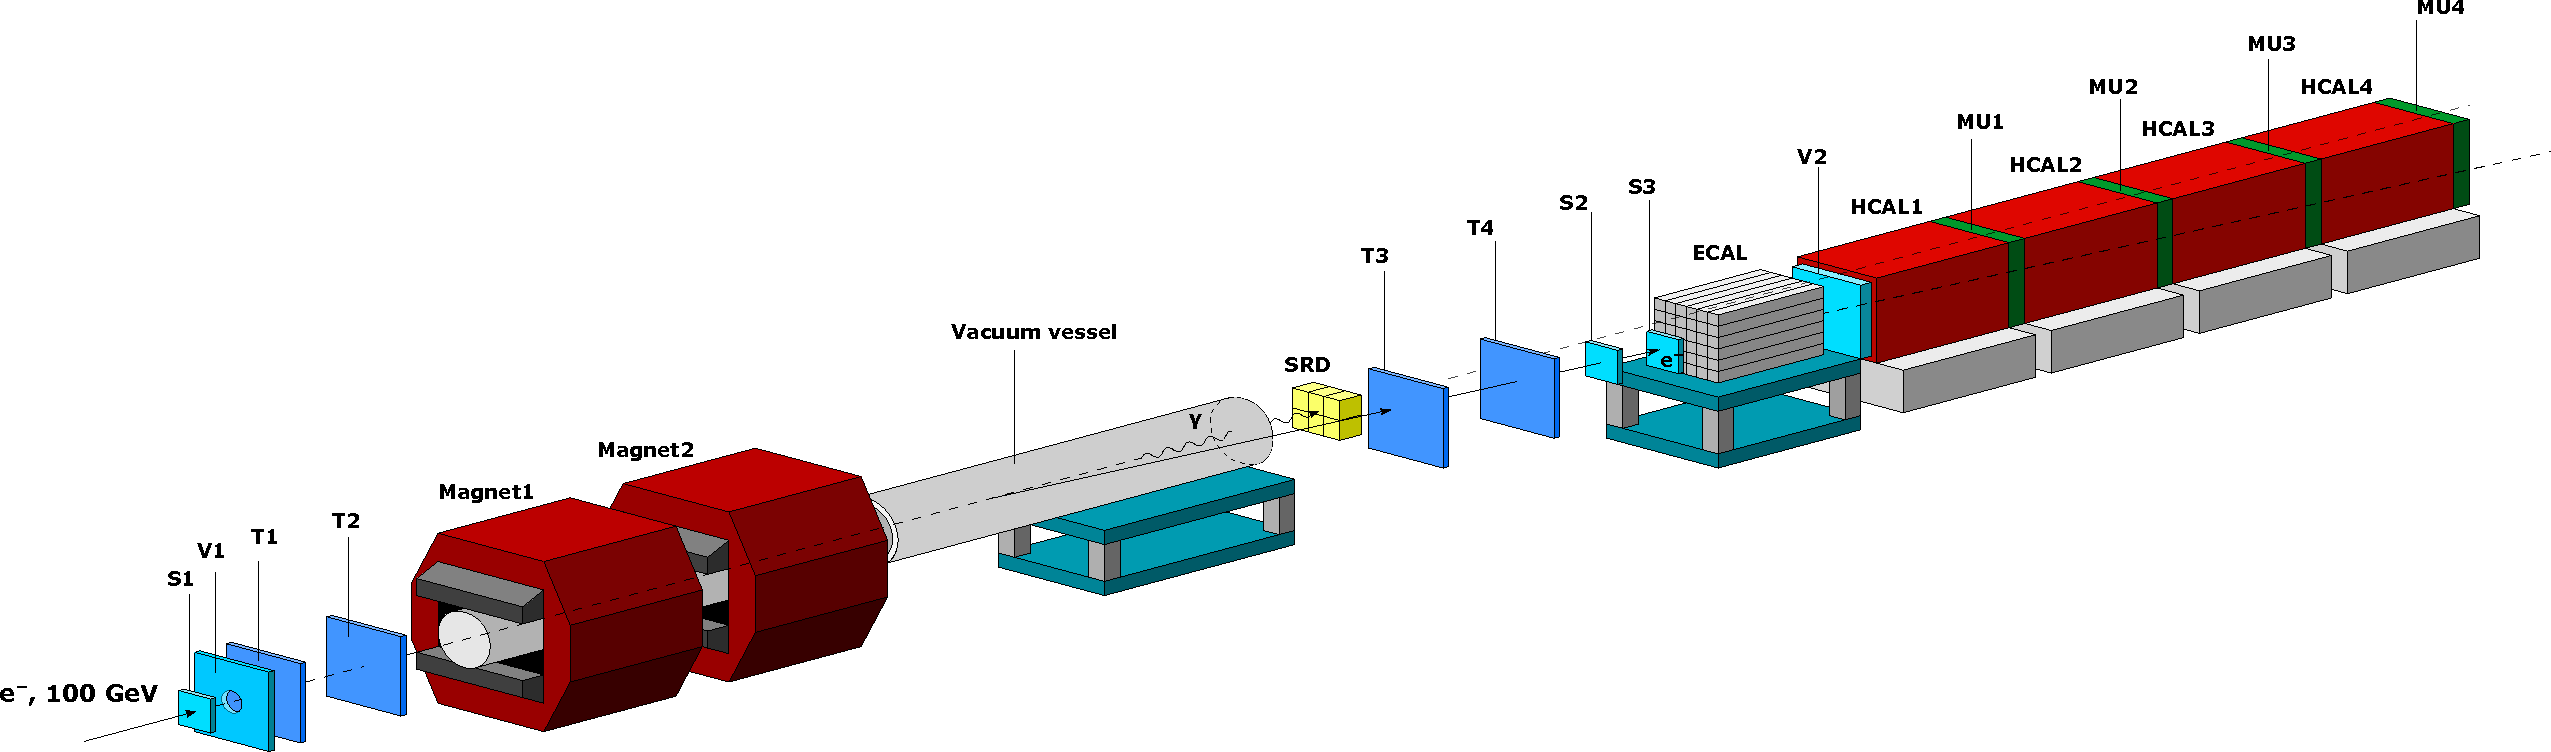
\includegraphics[width=\textwidth]{thesis_figures/Invisible_3d_setup.png}
\caption{Invisible mode setup~\cite{Banerjee:2016tad}}
\label{fig:Invisible_mode_setup}
\end{figure}

The Pierre Auger Observatory~\cite{} is the largest cosmic ray observatory in the world. Located outside Malargue in the Argentinian \textit{pampas} the observatory spans across an area of 3000k$m^2$. Originally conceptualized in the 1990s the Observatory was built in the early 2000s and fully completed in 2008. Geographically the site is located near the base of the Andes at an altitude of 1400m above sea level and across its whole span is relatively flat. The Observatory was designed to detect cosmic ray induced air showers having a primary energy from $10^{17}$eV to $10^{20}eV$ and beyond. It does so by identifying the EAS via two different complementary detecting components: \textit{Surface Detector} array (SD) and the \textit{Fluorescence Detector}(FD). A schematic o the observatory is shown in fig.~\ref{}. The SD consists of 1660 water Cherenkov tanks spread in a triangular grid with 1.5km spacing. The FD consists of four sites with 27 telescopes located at the edges of the ground array and overlooking the sky above. The Observatory also consists of various atmospheric monitoring devices such as LIDARs~\cite{}, laser facilities CLF and XLF~\cite{} and other weather sensors to constantly monitor the atmosphere which is important for FD operation. With the AugerPrime upgrade of the Observatory which is scheduled to be finished in 2024 two new detecting components are being added: The \textit{Radio Detector}(RD)~\cite{} and the \textit{Underground Muon Detector}(UMD)~\cite{}. The SD is also being upgraded with the addition of a scintillator on top of the tanks~\cite{}. Each individual component of the new upgrade is not discussed in detail since they are not used in the context of this thesis but only AugerPrime as a whole and its potential for detecting neutrinos at the Pierre Auger Observatory is discussed.

Eventhough, the primary objective of the Pierre Auger Observatory is UHECR physics it can also detect the neutrino induced EAS signature via both the SD and FD. The low neutrino interaction probability requires a detector which is always active. The high duty cycle of the SD $\approx 100$\% compared to a limited duty cycle of the FD $\approx 10-13$\% makes SD the more probable of the detector to detect neutrinos. This has already been shown in previous neutrino searches at Auger~\cite{} where the search with the SD provides the stringiest limits for neutrino searches at the Observatory~\cite{}. This chapter aims to provide a short review of the different components of the Observatory with a focus on the SD and its trigger system since it is the primary detector used for the analysis presented in this thesis. 

\section*{Fluorescence Detector}
\label{sec:Fl_det}
The Fluorescence Detector system at the Pierre Auger Observatory consists of an array of Fluorescence telescopes that are constantly looking inwards over the surface detector array trying to measure the nitrogen fluorescence induced by the EAS. The FD consists of 24 telescopes located at four different small hills( Coihueco, Los Morados, Loma Amarilla and Los Leones). The Coihueco site also consists of High Elevation Auger Telescopes (HEAT) which can be tilted upwards to extend the field of view at the Coiheuco site. Each of the 24 telescopes have a field of view of $30^{\circ} \times 30^{\circ}$ in azimuth and elevation. The combination of the telescopes gives a azimuth coverage of $180^{\circ}$. The HEAT telescopes can extend the field of view by a further $30^{\circ}$ in elevation. This gives a 100\% triggering efficiency for EAS above $10^{19}$eV for FD and above $10^{17}$eV with the inclusion of HEAT. Currently, the FD is always operated in combination with SD. The expected fluorescence yield   



\begin{figure}[t!]
\centering
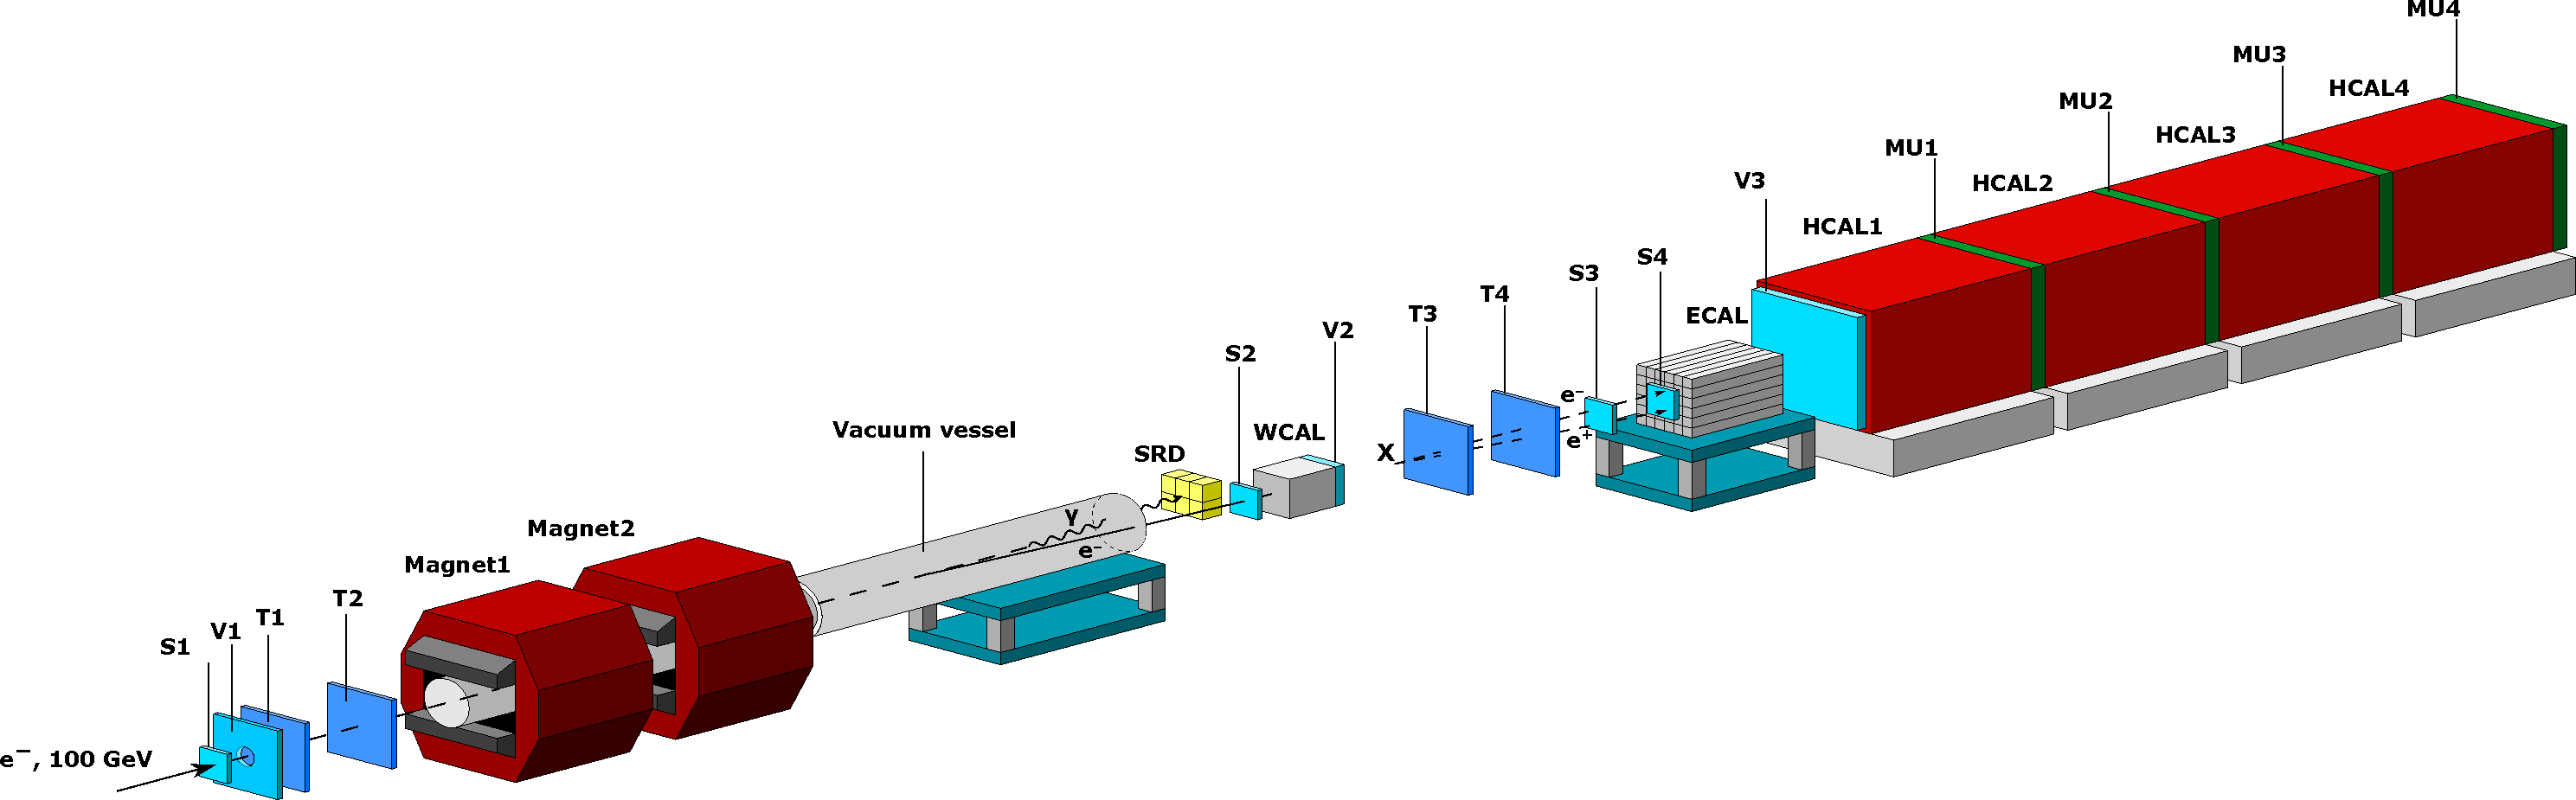
\includegraphics[width=\textwidth]{thesis_figures/Visible_3d_setup.png}
\caption{Visible mode setup 2017~\cite{Banerjee_2018}}
\label{fig:Visible_mode_setup}
\end{figure}

\begin{figure}[t!]
\centering
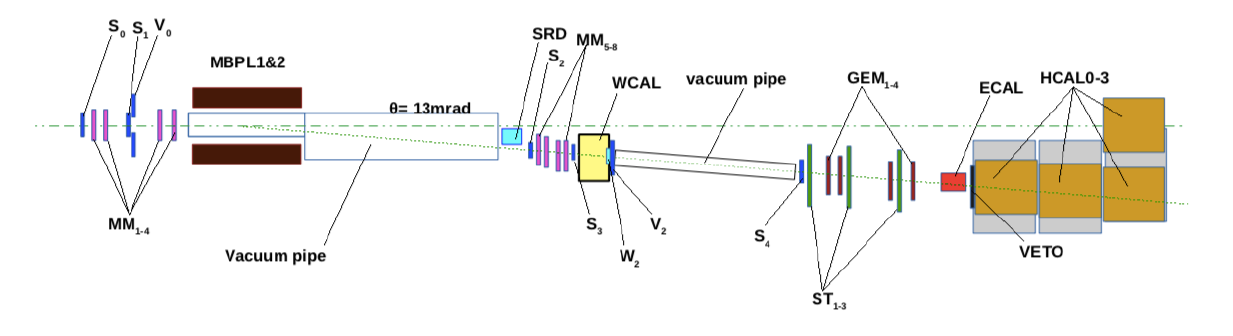
\includegraphics[width=\textwidth]{thesis_figures/visible_mode_newest.png}
\caption{Visible mode setup 2018-top view~\cite{Gninenko:2677228}}
\label{fig:Visible_mode_setup_side}
\end{figure}

The above setup works well for the \textit{invisible mode}($10^{-4} \lesssim \epsilon \lesssim 10^{-3}$, $m_{A'} \lesssim 1 \text{GeV}$) but requires modification for the search of $A'(X)$ in the \textit{visible mode}($10^{-4} \lesssim \epsilon \lesssim 10^{-3}$, $m_{A'} \lesssim 100 \text{MeV}$). To search for the visible decays a short tungsten calorimeter (WCAL) and a veto ($V_2$) were added right after the vacuum pipe and before the second set of tracking detectors (fig.(\ref{fig:Visible_mode_setup})). The size of the WCAL was selected so that the leakage of particles is small and the sensitivity to short lifetimes is maximized. The distance between the WCAL and the ECAL for the visible mode searches was slightly varied(2.5m->5.6m) between 2017 and 2018 which allowed for the installation of a 3.1m long vacuum tube to create better spacing between the ECAL and WCAL for a better angular resolution to increase the sensitivity to X17 bosons~\cite{Banerjee_2018}. A WCAL catcher was also installed in 2018 to prevent any leakage. Additionally the beam momentum was increased from 100GeV to 150 GeV in 2018 and one of the tracking station consisting of two MicroMegas (MM) was also shifted upstream of the WCAL. Counter ($W_2$) and straw detectors ($\text{ST}_{1-3}$) were also tested during the 2018 beam period(fig.(\ref{fig:Visible_mode_setup_side})). Both \textit{invisible} and \textit{visible} mode setups were also used to look for rare SM events that involve a photon decaying to a dimuon pair via bremsstrahlung $e^-Z\rightarrow e^-Z\gamma;\gamma\rightarrow \mu^{+} \mu^{-} $. Comparing these rare events, which were obtained from real data, to our Monte Carlo(MC) simulated sample helped in estimating the validity and efficiency of our MC simulation~\cite{Gninenko:2677228}.

In summary, NA64 tries to estimate and tag the beam $e^-s$ using a combination of trackers, SRD and ECAL/WCAL, uses the said ECAL/WCAL as an active target and then collects the residue of the interaction in the downstream HCAL/ECAL+HCAL. It also utilizes the hard bremsstrahlung photon to dimuon conversion as a measuring stick for the reliability of the MC simulations. The reactions of interest were attempted to be observed with a combination of hardware and software triggers depending on the expected signature of the decay mode for $A'$.

\textbf{Invisible Mode:}
$A'\rightarrow \chi \overline{\chi}$ signature:
\begin{flalign*}
  Beam(p\simeq 100~\text{GeV}),\\
  E_{ECAL+PS}(< 100~\text{GeV}),\\
  V_2(< E^{th}_{V}\simeq 1~\text{MIP}),\\
  E_{HCAL}(< E^{th}_{HCAL}\simeq 1~\text{GeV}).
\end{flalign*}

\textbf{Visible Mode:}
$A'\rightarrow e^+ e^-$ signature:
\begin{flalign*}
  Beam(p\simeq 150~\text{GeV}), \\
  E_{WCAL}(< 150~\text{GeV}), \\
  E_{WCAL+ECAL+PS}(\simeq 150~\text{GeV}), \\
  V_2(> E^{th}_{V}\simeq 1~\text{MIP}), \\
  V_3(< E^{th}_{V}), \\
  E_{HCAL}(< E^{th}_{HCAL}\simeq 1~\text{GeV}).
\end{flalign*}







%%% Local Variables:
%%% mode: latex
%%% TeX-master: "mythesis"
%%% End:
